% !TEX root = main.tex

\chapter{試料構造と測定方法}%================================
%\label{chap:simulation}

\section{はじめに}%========================================
本研究ではInGaAs/GaAs多重量子井戸・ファブリーペロー型の半導体レーザーをデザインした。本章では2.2節でそのエピ構造とデバイス化のためのプロセスについて、2.3節で測定手法について述べる。
\section{試料作製}%========================================
本研究では活性層にInGaAs/GaAs多重量子井戸を持つウエハをデザインした。本2.2節ではデザインと測定するためのデバイス化について述べる。ウエハの結晶成長はNTT-ATおよび台湾の会社?に依頼した。結晶成長また後述のリッジ加工プロセスやコンタクトメタル蒸着はNTT-ATに依頼した。

\subsection{試料構造}%=====================================
まずはエピウエハ構造について述べる。量子井戸の周期は3周期と10周期の2種類である。それぞれのエピ構造を図\ref{fig:sample_structure}に示す。nタイプGaAs基板の上にバッファ層が丸々nm,その後n-AlGaSがどうたらこうたらSCH層がどうたらこうたら.。バンドギャップの図があると良い屈折率とかも
\begin{figure}[t]
	\centering
	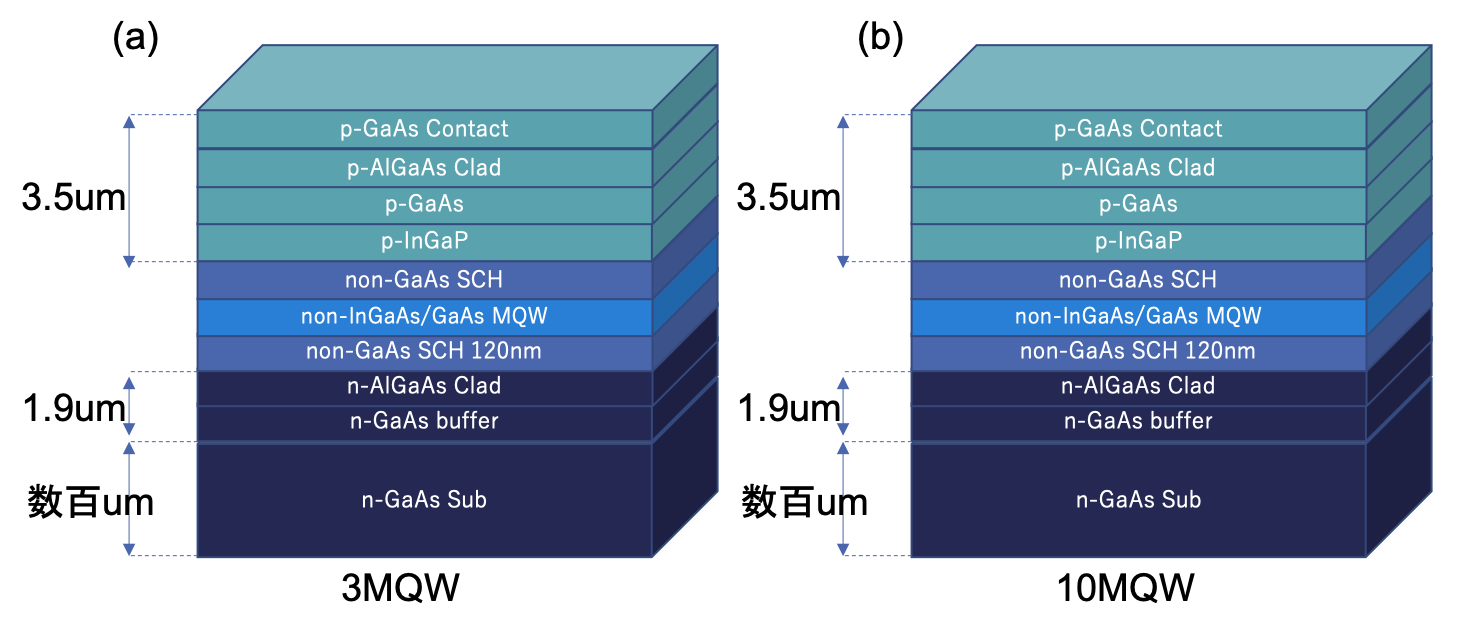
\includegraphics[width=15cm]{figure/fig_2_1_sample_structure}
	\caption{エピウエハ構造}
	\label{fig_2_1_sample_structure}
\end{figure}

\newpage
\subsection{ブロードコンタクトレーザー}%=======================
結晶成長の後n側とp側にコンタクトメタルの蒸着を行った。p側の原子はなになに、n側はなになにである。劈開面は001?とかなんとか
ブロードコンタクトレーザーとは光導波路を形成せずバー(棒)のままのレーザーである。プロセスを簡略化することで早く測定を行うことを目的とした。ウエハの評価測定のために用いた。図\ref{fig:sample_broadcontact}に模式図を示す。図\ref{fig:sample_broadcontact}の上から下に向かって電流が流れ、活性層でキャリアの再結合が起き発光が起こる。また図の手前と奥の劈開面でファブリーペロー共振器を形成しており、反転分布となっているときに光がそこを往復することで誘導放出が起き発振し、紙面の手前と奥方向に(軸を用意した方がいいか?)この文章だと絵をバーっぽくした方がいいか?共振器長は500,1000,2000umの3種類を作製した。また電極パッド幅は3,5,10,30,50,100,300umの6種類を作製した。

\begin{figure}[t]
	\centering
	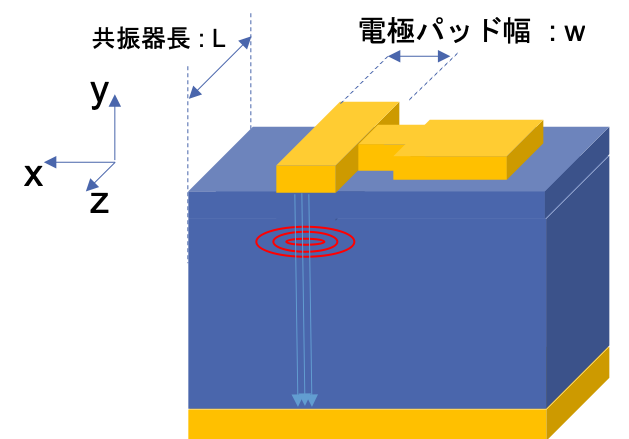
\includegraphics[width=10cm]{figure/fig_2_1_broadcontact.png}
	\caption{ブロードコンタクレーザー}
	\label{fig:sample_broadcontact}
\end{figure}

\begin{figure}[t]
	\centering
	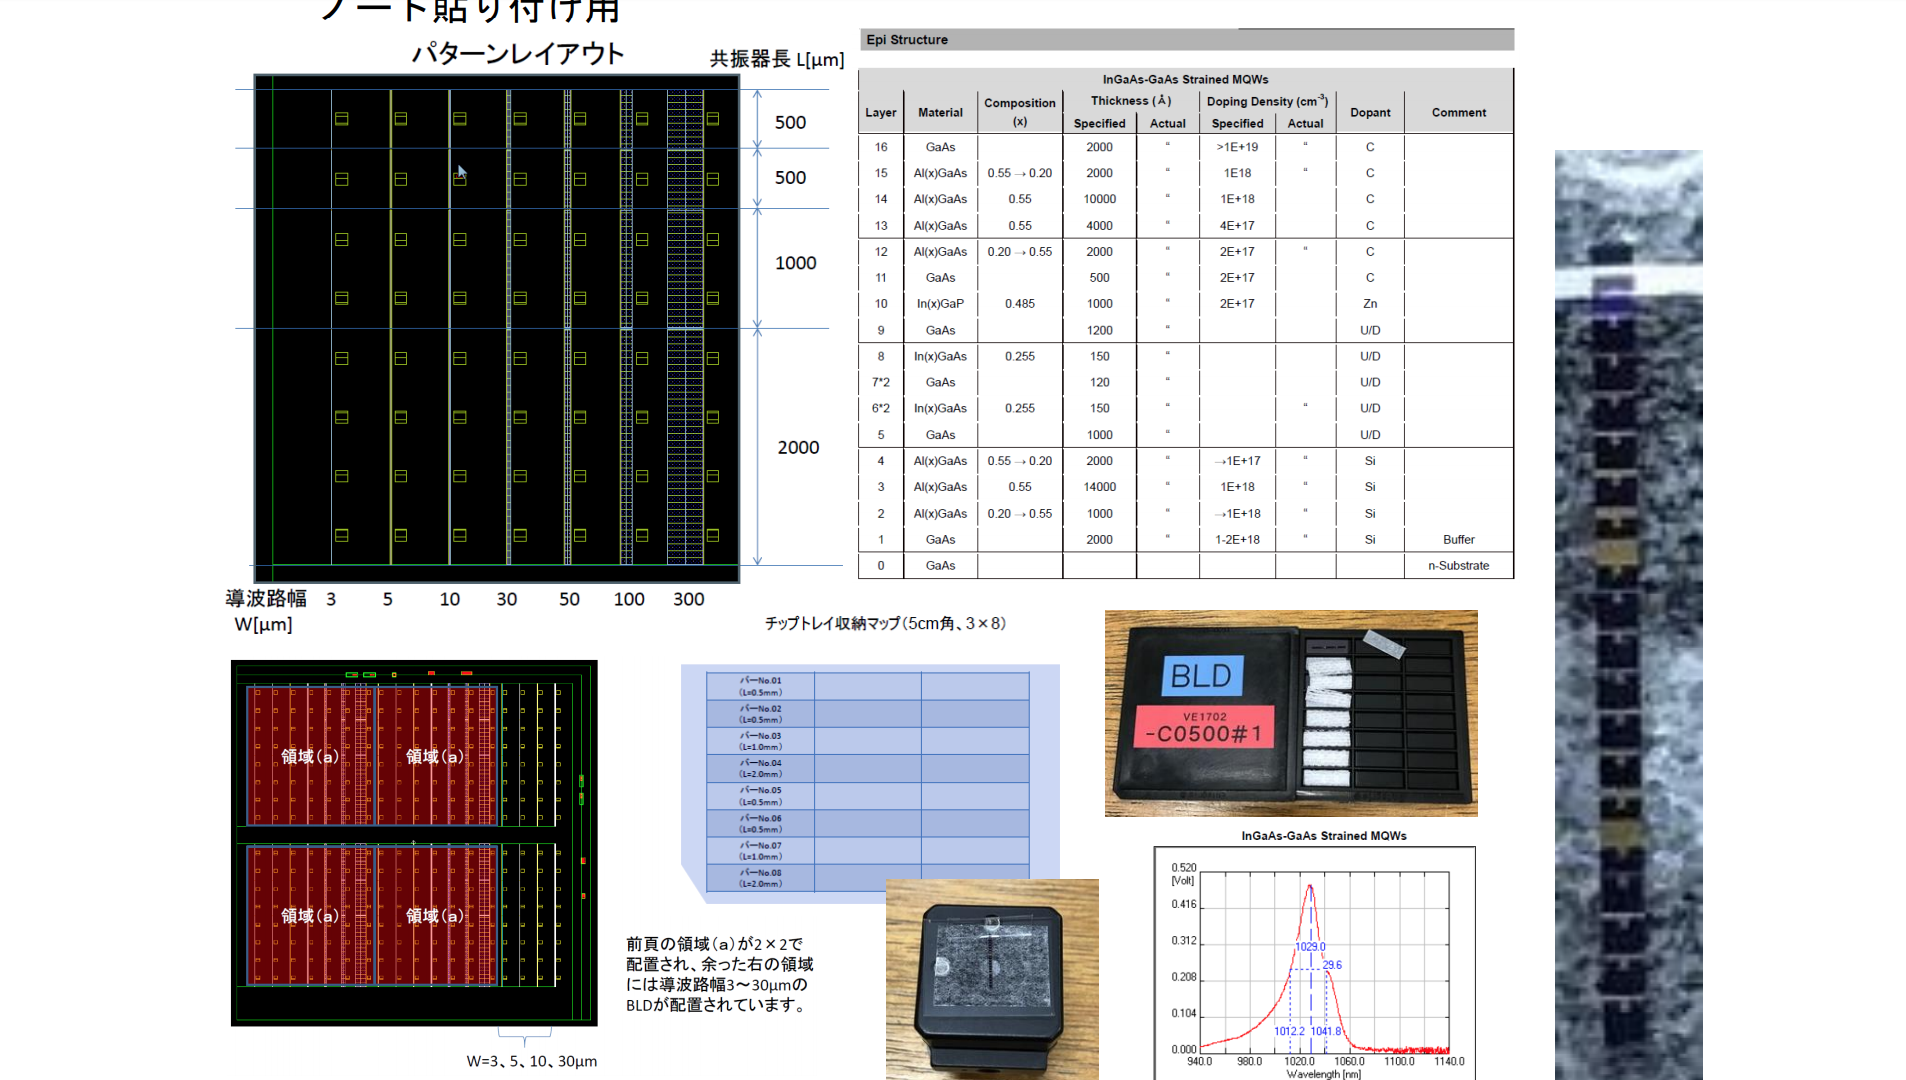
\includegraphics[width=10cm]{figure/fig_2_1_broadcontact_memo.png}
	\caption{ブロードコンタクレーザーめも}
	\label{fig:sample_broadcontact_memo}
\end{figure}

\subsection{リッジ導波路型レーザー}%==========================
次にリッジ導波路型レーザーについて述べる。その模式図を図\ref{fig_2_1_ridge}に示す。エピウエハ作製後p側クラッド層を活性層直上までエッチングすることで光導波路を形成している。横方向の光閉じ込めが大きくなるため、キャリアと光の重なりが大きくなるため利得を大きく?することができる。参考文献欲しい。最終的に利得スイッチング動作を試みるデバイスである。
共振器長は100,200,300,400,500,1000um,リッジ幅は1.5um,2.5umのものを作製した。
\begin{figure}[t]
	\centering
	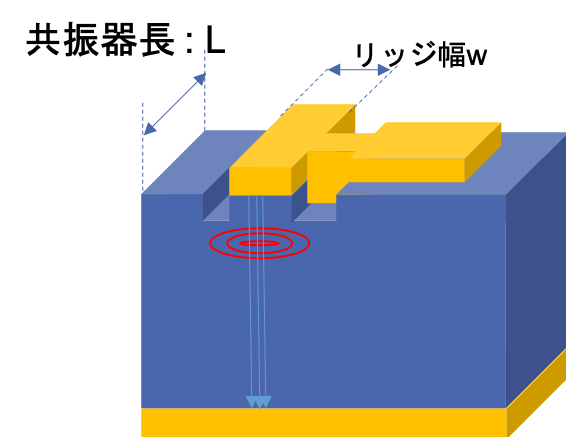
\includegraphics[width=10cm]{figure/fig_2_1_ridge.png}
	\caption{リッジ導波路型レーザー}
	\label{fig_2_1_ridge}
\end{figure}

\subsection{マウント(ダイボンディング??)}%======================
作製したブロードコンタクトレーザーバーおよびリッジ導波路型レーザーを電流注入実験を行うためにマウントを行なった。それぞれ図に示す。\\
 レーザーバーはAlN基板にAnSnメッキを施してあるサブマウント(....社製)にダイボンディングした。ブロードコンタクトレーザーはダイボンディングしてなかったっけ?そういえば
この状態で試料上面の電極をプローバー(先端の径...程度の金属の針)でさわり、電流を流した。一本のバーに5個程度の素子があるので測定が終わったら次々とプローバーの触る箇所をかえていけば速やかに測定を続けることができる。\\
 一方リッジ導波路型レーザーの一部は利得スイッチング動作実験を行うために高速応答が期待できるようにマウントした。Transistor Outlineパッケージと呼ばれる缶状の金属にマウントを行った。....社製のCANを用いた。その際レーザーバーをさらに分割し1つ1つの素子に分離した。分離した素子をAnSn共晶材あるいはエポキシを用いてCANにダイボンディングし、金線をワイヤーボンディングマシンで配線した。


\begin{figure}[t]
	\centering
	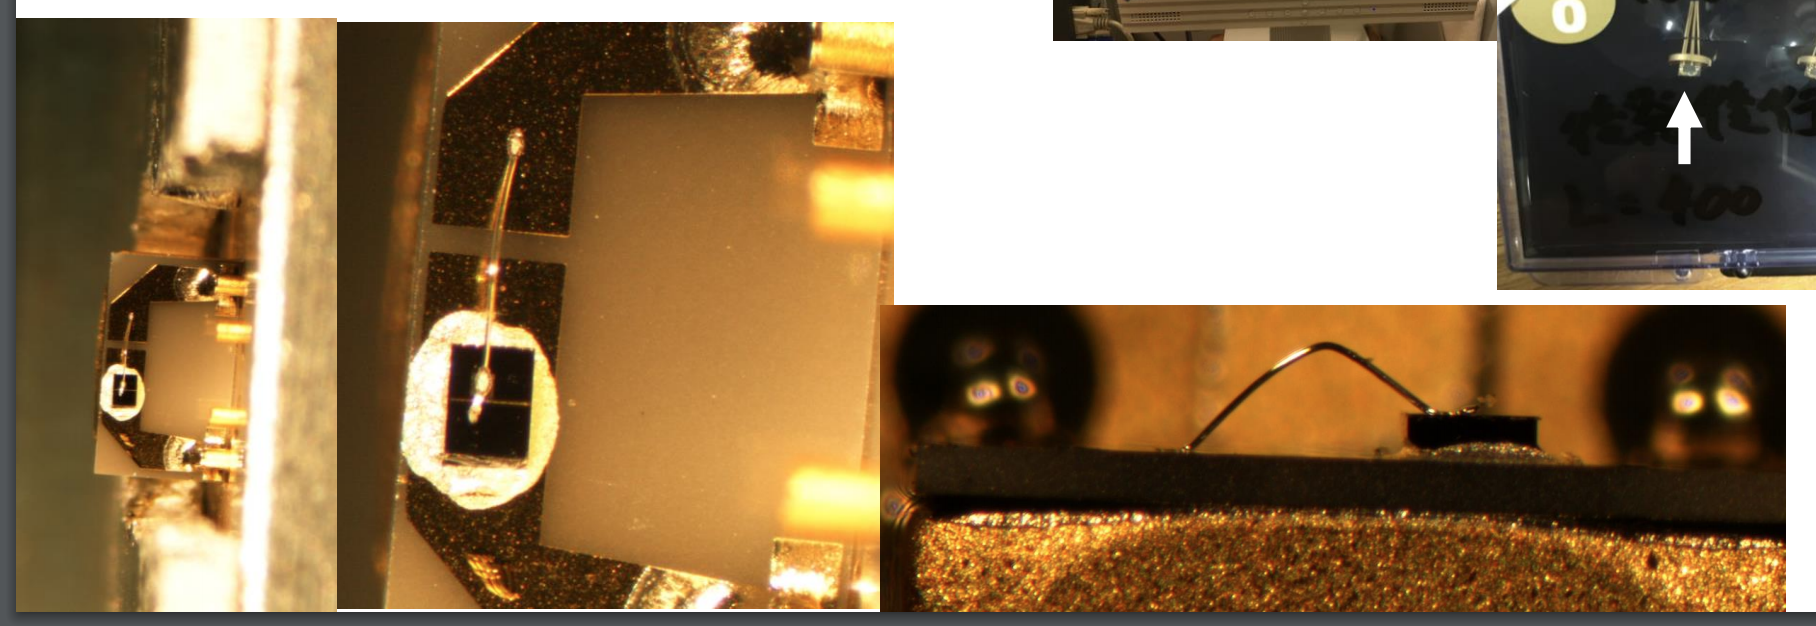
\includegraphics[width=15cm]{figure/fig_2_1_mount.png}
	\caption{測定デバイス外観}
	\label{fig_2_1_mount}
\end{figure}

\section{測定方法}%========================================
本研究ではエピウエハの品質評価のための測定と利得スイッチング動作を起こしデバイスの高速特性を評価するための測定を行った。
\subsection{定常電流注入による測定実験}%=======================
まずエピウエハの品質を調べるために定常電流を注入する実験を行った。発振閾値電流や発振閾値電流密度などの基本的な物性パラメータを見積もることができる。
実験系を図\ref{fig:IL}に示す。パルスジェネレータから数usパルスを数ms周期で発生させ、試料に注入する。ここでマイクロ秒程度のパルスは試料の中での発光過程やその他の物理現象の時間オーダーに対して十分長く、定常電流とみなすことができる。DC電流では熱の影響が大きくなってしまい試料が壊れてしまう恐れがあるため。Duty比(パルス幅と繰り返し周期の比)を1:1000程度に設定して実験を行った。試料からの発光強度を光パワーメータで測定した。また、回路に試料と直列に抵抗(22.4オーム)を入れ、そこにかかる電圧をモニタすることで流れる電流量および、試料にかかる電圧を測定した。試料にかかる電圧は回路全体にかかる電圧と抵抗にかかる電圧の差を取ることにより算出した。
\begin{figure}[htbp]
	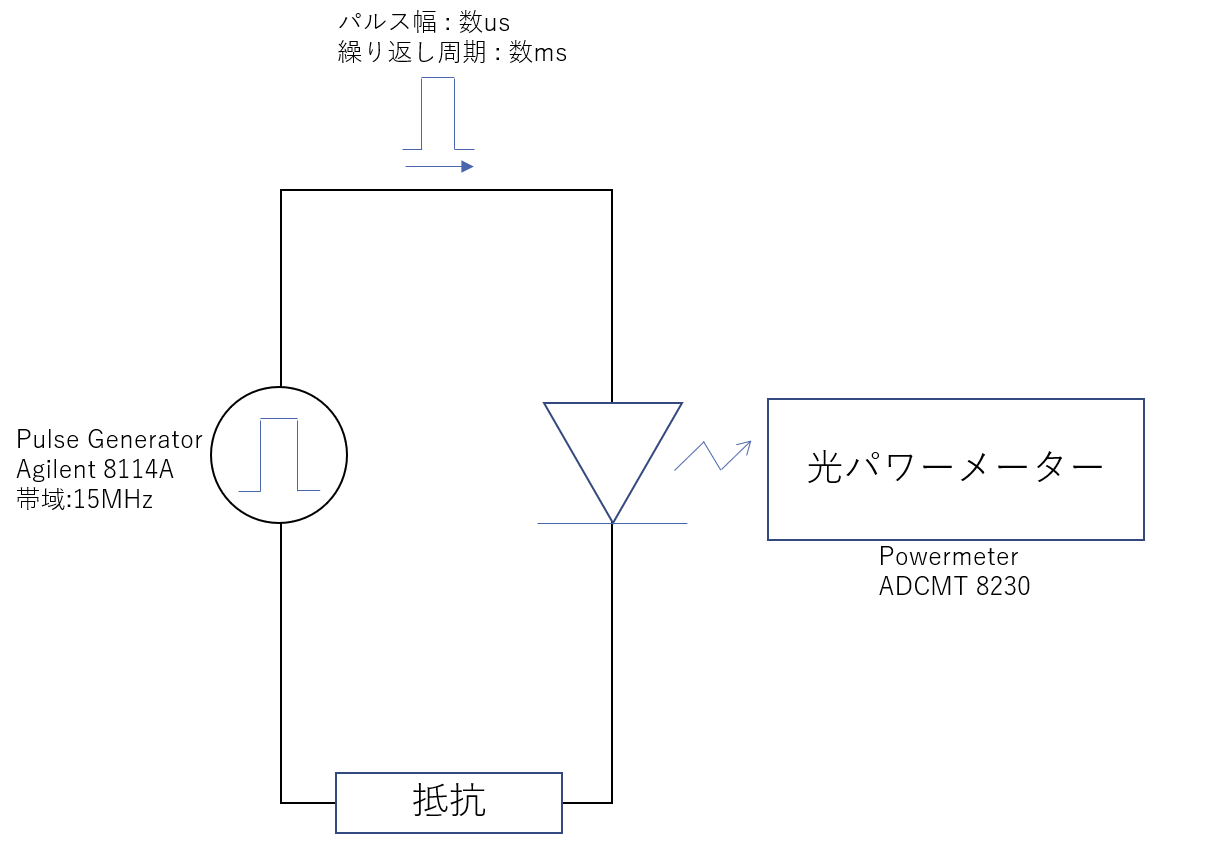
\includegraphics[width=15cm]{figure/fig_2_2_IL_setup.png}
	\caption{IL実験系}
	\label{fig_2_2_IL_setup}
\end{figure}

\subsection{電流注入利得スイッチング実験}%======================
ナノ秒程度の短いパルス電圧を引火することで利得スイッチング動作を起こし測定を行なった。その実験系の回路図を図\ref{fig:GS_setup}に示す。パルスジェネレータから同軸ケーブルを介して試料へ電気パルスが印加される。パルスジェネレータからで生成された電圧パルスは可変抵抗、RFアンプで増幅されデバイスへと印可される。試料からの発光は対物レンズでコリメートされ、非球面レンズで光ファイバーに集光される。その後フォトダイオードで検出しその電圧を高速オシロスコープでモニタした。

PDの分解能について記述!
\begin{figure}[htbp]
	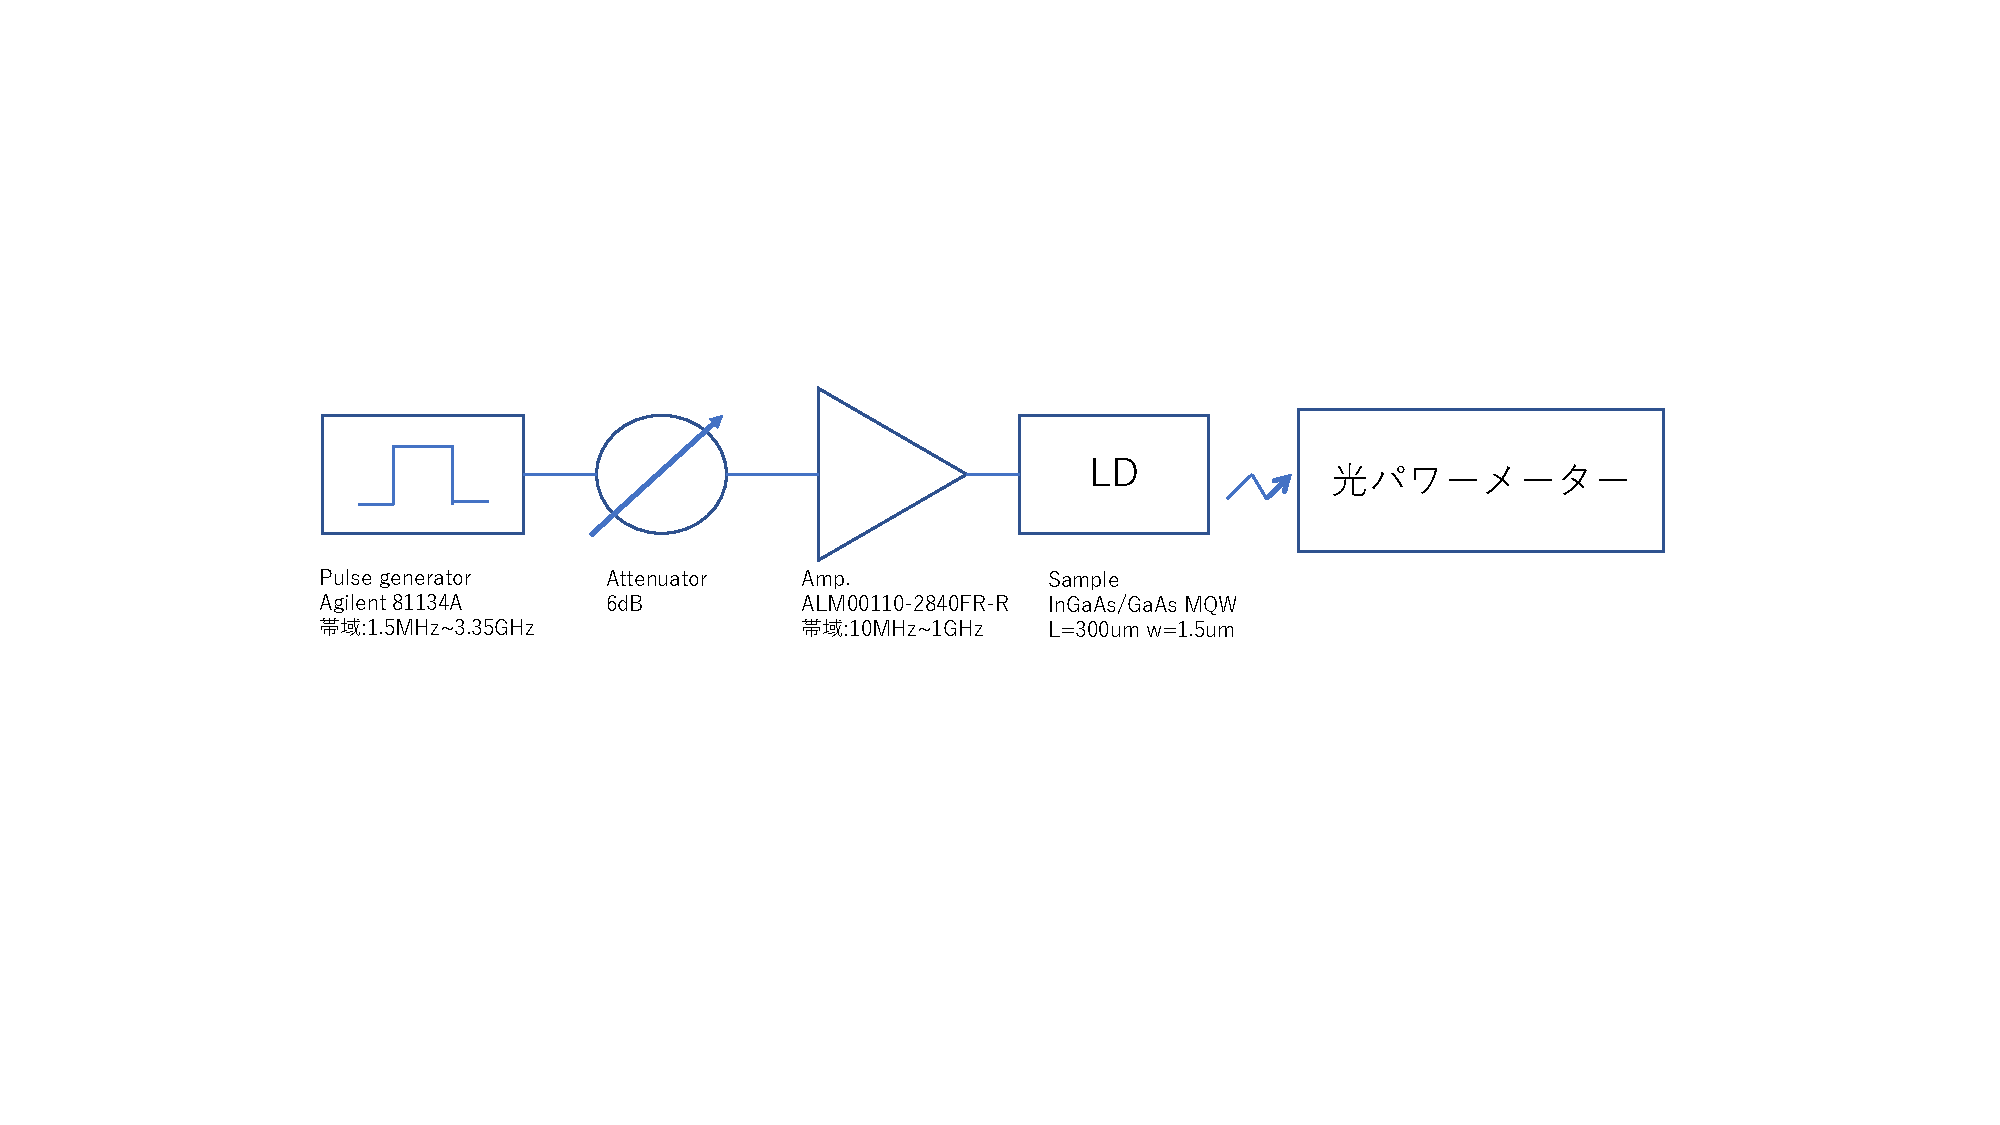
\includegraphics[width=15cm]{figure/fig_2_3_1_01_GS_setup.pdf}
	\caption{GS実験系}
	\label{fig:GS_setup}
\end{figure}

